\section{Statistical Analysis} \label{section:higgs_analysis}

\subsection{Signal Modeling} \label{subsection:higgs_analysis_signal}
%
% Outline:
% - General Description of Signal Modeling
% - Choice of Pdfs
% - Procedure for Building/Fitting/Extracting Model Parameters
% - Normalization
%

%
% General Description
%
To be able to judge/draw conclusions about possible excess of events, due to the SM Higgs Boson, we ought to build a model aiming to explain the to be observed excess. Given we are looking for a bump-like structure near the Higgs Boson Mass, it is natural to model this excess via a composition of Gaussian functions. Each category and production process has been treated individually/separately and only depends on the Higgs Boson Mass and nuisance parameters to be described further. In the modeling we perform, we follow a similar approach that has previously been described in the Run~I $H\rightarrow\gamma\gamma$ analysis \cite{CMS-PAS-HIG-13-001,CMS_AN_2013-253}.

The Signal Model for the Higgs boson like signal accounts for both shape and normalization, fully parametric in $\mH$, and in the nuisance parameters described in section FIXME. %% ~\ref{xxx}{\bfseries}.

\begin{align}
   \label{eq:higgs_signalmodel_DoubleGaus}
   S(x,\mH, \theta) &= f \mathcal{N}_{1}(x, \mu_{1}, \sigma_{1}) + (1-f)  \mathcal{N}_{2}(x, \mu_{2}, \sigma_{2}) \\
   \label{eq:higgs_signalmodel_TripleGaus}
   S(x,\mH, \theta) &= f_{1} \mathcal{N}_{1}(x, \mu_{1}, \sigma_{1}) + (1-f_{1}) \left(f_{2} \mathcal{N}_{2}(x, \mu_{2}, \sigma_{2}) + (1-f_{2}) \mathcal{N}_{3}(x, \mu_{3}, \sigma_{3})\right)
\end{align}

where $\mathcal{N}(x,0,1)$ is a normal distribution, $\mu_i(\mH,\theta), \sigma_i(\mH,\theta)$ are respectively the mean and sigma of each gaussian, $x$ is the reconstructed invariant mass of the two muons (\mmm), and $\theta$ is the list of parametric nuisances.

%
% Choice of Pdfs
%
Both double eq~\ref{eq:higgs_signalmodel_DoubleGaus} and triple eq~\ref{eq:higgs_signalmodel_TripleGaus} Gaussian forms were tested.
The main reason for extending the form up to triple Gaussian (w.r.t. Run~I)
is to be able to pick up both the possible mass shift due to FSR and accomodate the broadening due to detector resolution effects.

%
% Procedure
%
For each category and each production process (ggH, qqH, WPlusH, WMinusH, ZH, ttH) , all of the signal parameters are derived by fitting a given model (Double eq~\ref{eq:higgs_signalmodel_DoubleGaus} or Triple eq~\ref{eq:higgs_signalmodel_TripleGaus} Gaus) to the dimuon invariant mass $\mmm$ spectrum obtained from the MC signal samples (described in FIXME %% section~\ref{sec:mc}
) being subject to the same event selection as data (section~\ref{section:higgs_selections}).
For the purpose of testing various Higgs Boson Mass hypotheses, three mass points ($\mH=120\,\gev$, $125\,\gev$, $130\,\gev$) were used, which allows us to interpolate in between and probe any mass in the range $[120, 130]\,\gev$.

The procedure to extract model parameters from the signal MC goes as following:
\begin{itemize}
    \item For a given category and production process
    \item Start with the invariant mass spectrum for $\mH$ of $120\,\gev$ and perform a binned maximum likelihood fit using initial default parameters.
    \item Proceed to next point in mass ($\mH$ of 125 GeV), by using the same fitted resolution ($\sigma_{i}$) from the previous fit ($\mH= 120\gev$) and shifted scale ($\mu_{i}$), by the mass difference, parameters as initial guesses.
        Perform the Maxlikelihood Fit and extract the parameters.
    \item Proceed to the $\mH$ of $130\,\gev$ and perform the same procedure as for $125\,GeV$.
    \item Each parameter $\mu_{i}, \sigma_{i}, f_{i}$ can be now interpolated across the mass points, using spline function.
    \item At this point, we have all the parameters ($\sigma_{i}$, $\mu_{i}$, $f_{i}$) be functions of $\mH$.
\end{itemize}

%% Fig.~\ref{sigmodel:gaus}
Figure~\ref{fig:higgs_signalmodel_signalExamples} shows an example of fit with three gaussians on the left, an example of interpolation on the center, and an example of efficiency times acceptance on the right. All plots are available in FIXME.
%% Appendix~XXX.

\begin{figure}[hbp]
    \centering
    \subfigure[]{
        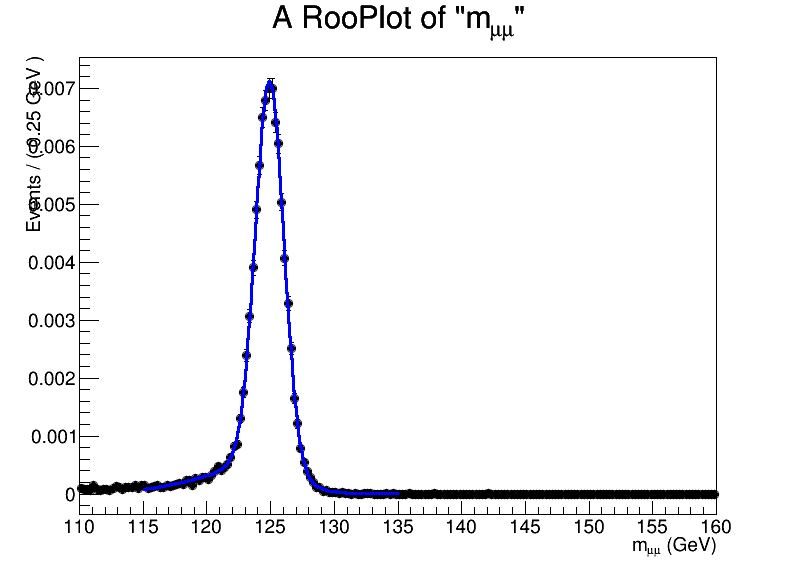
\includegraphics[width=0.3\textwidth]{figures/ch_higgs/signalmodel/baseline/signalFit__01JetsTightBB__125__GluGlu__TripleGaus__default.png}
    }~
    \subfigure[]{
        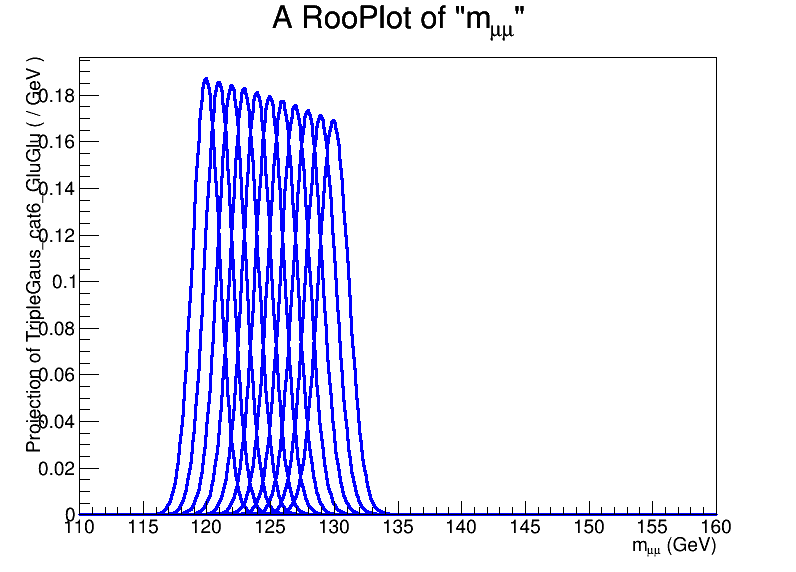
\includegraphics[width=0.3\textwidth]{figures/ch_higgs/signalmodel/baseline/signalFitInterpolationWithSpline__01JetsTightBB__GluGlu__TripleGaus__.png}
    }
    \caption{(a) Signal Fit. (b) Signal Fits and Interpolations}
    \label{fig:higgs_signalmodel_signalExamples}
 \end{figure}

%
% Normalization
%
The last missing piece for Signal Model building is the normalization.
Given a dimuon invariant mass distribution for a particular category for a particular production process,
the expected yields can be expressed as in equation~\ref{eq:higgs_signalmodel_expectedYield}.

\begin{align}
        %\label{eq:signalNormalization}
        %\text{Norm} = {\frac{\mathcal{L} \sigma \mathcal{B}(\Htomm)}{N_{gen}}} \\
        \label{eq:higgs_signalmodel_expectedYield}
        %\text{Yield} = {Norm \times \sum_{bins}^{} N_{i}}
        %\label{eq:efficienceAcceptance}
        \text{Yield} = \mathcal{L}\,\sigma(pp\rightarrow H)\, \mathcal{B}(\Htomm) \, \varepsilon A
\end{align}

The production cross sections ($\sigma(pp\rightarrow H+X)$) for each process and the branching ratio of the Higgs boson to decay into a muon pair ($\mathcal{B}(\Htomm)$) are taken from the Yellow~Report~4 \cite{YR4} as centrally provided in {\it combine} (see more on this in section%~\ref{combine_tool}).

Effieciency times acceptance ($\varepsilon A$) is computed using the MC sample information as
\begin{align}
\varepsilon A = \frac{1}{N}\sum w_i r_{i} \text{sf}_i \mathbf{1}_\textup{catX}
\end{align}

where $w_i$ is the generator weight, $r_i$ is the ``pileup reiweighting'' factor used to match the truth pu distribution injected in the MC to the one measured in data,
$\text{sf}_i$ is the total scale factor associated to the event,  {\bf FIXME describe more or refer to something.}
$\mathbf{1}_\textup{catX}$ is the identity function on the classification ($1$ if the event is in the category, $0$ otherwise),
and $N$ is the total normalization factor at generator level $N=\sum w_i$, where the sums runs over the entire MC dataset.

%whose entries correspond to the weighted number of events ($\rm{N_{i}}$) per bin,
%the overall normalization is computed according to eq~\ref{eq:signalNormalization}.
%which we can rewrite in terms of efficience and acceptance as in eq~\ref{eq:efficienceAcceptance}.

%Eq~\ref{eq:efficienceAcceptance} demonstrates three different pieces that will come together later on in section~\ref{combine_tool} : Integrated Luminosity, Cross-Section ($\sigma$) and Branching Ratio, and $\epsilon A$.
%For the purpose of modeling, Integrated Luminosity is a single number that is measured centrally; $\epsilon A$ is the normalization we extract from SM Signal Samples and they come in as functions of $\rm{m_{H}}$. Finally, for Cross-Sections and Branching Ratios, which are also functions of $\rm{m_{H}}$, we use centrally provided values by Combine (see more on this in section~\ref{combine_tool}).

\subsection{Background Modeling} \label{subsection:higgs_analysis_background}
%
% Outline:
% - Motivation
% - General Description of Background Modeling
% - Choice of Pdfs/bin granularity/mass range
% - Physics Motivated Models
% - Polynomial-like Families and F-Test
% - RooMultiPdf and combining multiple models
% - All of the parameters are floatin! Normalization as well!
%
Given highly dominant nature of background processes, it is important to properly model the background shape as that is the biggest contributor for any physical quantity of interest that we are to compute. In general, our background can be described by means of falling exponential with some polynomial contribution.

% Models: Physcs Motivated Models and Polynomial-like Families
For the purpose of modeling, we identify two classes of models that we consider: physics motivated models and families of models that are order-dependent (polynomials, sum of exponentials). The first class contains several pdfs whose  functional forms are driven by the knowledge of background processes contributing the most (Drell-Yan, ttbar). All of these shapes have been used for fitting the FEWZ generated mass shapes (more on this in appendix) and the fitted values for the parameters have been used as initial guesses for the Modeling Procedure. Second class of functions we consider comes from general families which are, in principle, capable of describing any functional form by incorporating more and more orders. Here, we consider several families, Bernstein, Power Law, Sum of Exponentials.


\begin{center}
    \begin{equation}
        \label{eq:higgs_backgroundmodel_ExpPol2}
        ExpPolynomial: {B(x)} = {e^{a_{1}x + a_{2}x^2}}
    \end{equation}
    \begin{equation}
        \label{eq:higgs_backgroundmodel_BWZ}
        BWZ: {B(x)} = {\frac{e^{ax}\sigma_{z}}{(x-\mu_{z})^2 + (\frac{\sigma_{z}}{2})^2}}
     \end{equation}
     \begin{equation}
        \label{eq:higgs_backgroundmodel_BWZRedux}
        BWZRedux: {B(x)} = {\frac{e^{a_{2}x + a_{3}x^2}}{(x-\mu_{z})^{a_{1}} + (\frac{2.5}{2})^{a_{1}}}}
     \end{equation}
     \begin{equation}
        \label{eq:higgs_backgroundmodel_BWZGamma}
        BWZGamma: {B(x)} = {f\frac{e^{ax}\sigma_{z}}{(x-\mu_{z})^2 + (\frac{\sigma_{z}}{2})^2} + (1-f)\frac{e^{ax}}{x^2}}
     \end{equation}
\end{center}

\begin{center}
    \begin{equation}
        \label{eq:higgs_backgroundmodel_Bernstein}
        Bernsteins: {B(x)} = {\sum_{i=0}^{n} \alpha_i[\binom{n}{i}x^{i}(1-x)^{n-i}]}
    \end{equation}
    \begin{equation}
        \label{eq:higgs_backgroundmodel_SumExponentials}
        SumExponentials: {B(x)} = {\sum_{i=1}^{n} \beta_{i}e^{\alpha_{i}x}}
    \end{equation}
    \begin{equation}
        \label{eq:higgs_backgroundmodel_SumPowers}
        SumPowers: {B(x)} = {\sum_{i=1}^{n} \beta_{i}x^{\alpha_{i}}}
    \end{equation}
    \begin{equation}
        \label{eq:higgs_backgroundmodel_Laurent}
        LaurentSeries: {B(x)} = {\sum_{i} \alpha_{i}x^{i}}
    \end{equation}
\end{center}

Figure~\ref{fig:higgs_backgroundmodel_exampleModels} shows several examples of background only fits to the data for various hypothetical functional forms. From left to right, we have functions being fit for the mass ranges [110, 160] GeV, [110, 200] GeV and [110, 250] GeV. For the full list of those, please refer to Appendix \textbf{FIXME}.

\begin{figure}[hbp]
     \centering
     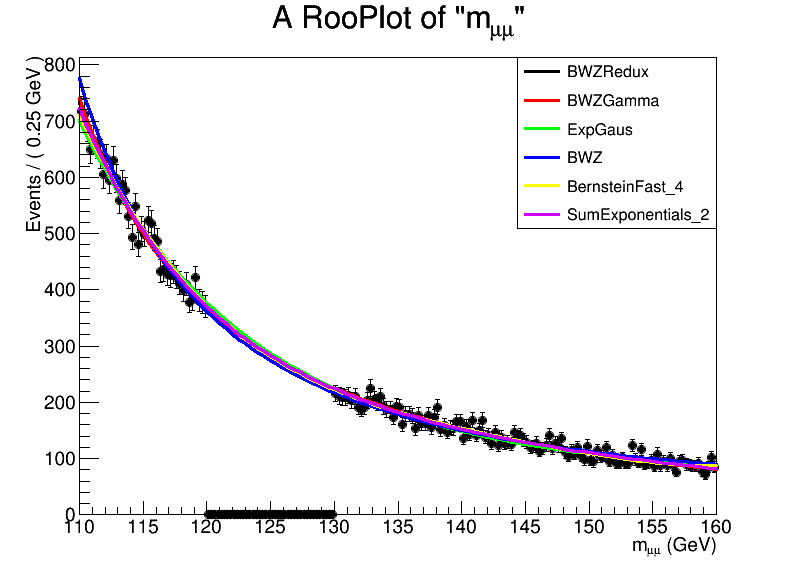
\includegraphics[width=0.3\textwidth]{figures/ch_higgs/backgroundmodel/baseline_110to160_p25GeV/backgroundFits__01JetsTightBB__bkgModels.png}
     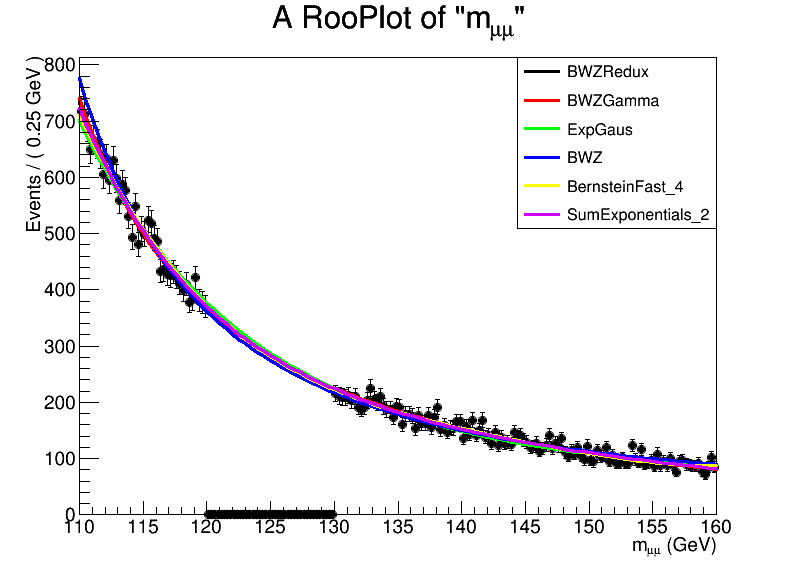
\includegraphics[width=0.3\textwidth]{figures/ch_higgs/backgroundmodel/baseline_110to160_p25GeV/backgroundFits__01JetsTightBB__bkgModels.png}
     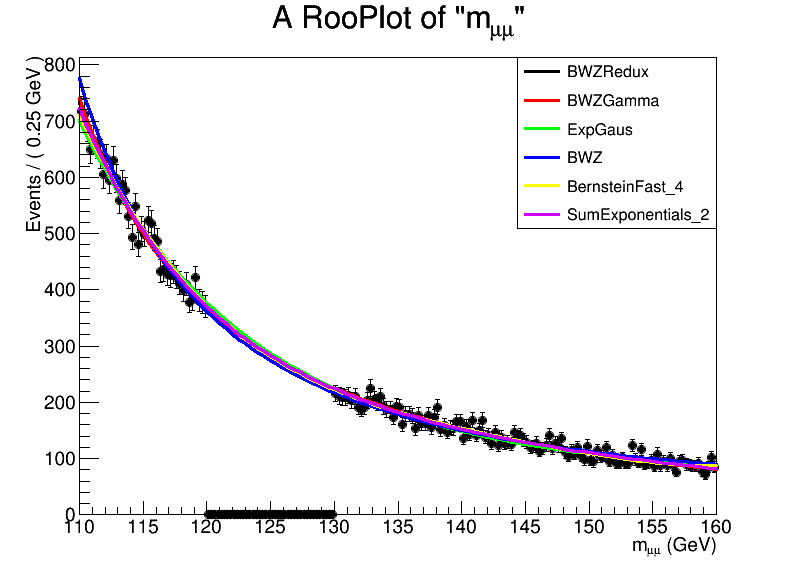
\includegraphics[width=0.3\textwidth]{figures/ch_higgs/backgroundmodel/baseline_110to160_p25GeV/backgroundFits__01JetsTightBB__bkgModels.png}
     \caption{}
     \label{fig:higgs_backgroundmodel_exampleModels}
 \end{figure}

The background modeling procedure involves the construction of an envelope (RooMultiPdf) of pdfs that can either be used individually or altogether for the purpose of Fitting or Limits Extraction. For the physics motivated functions, we simply perform the Maximum Likelihood Fit and insert that model into the envelope. However, for the order-dependent families, the procedure is a bit more involved, given that we are to select a model of certain order. The technique for selecting a particular order from a given family is the F-Test and goes as following:

\begin{itemize}
    \item For a given category and for a particular family
    \item Our hypothesis: order n is the true order. To reject this hypothesis, we have to be at least 95\% confident rejecting it - $p(\chi^2, ndf) < 5\%$
    \item Perform the background only fit for orders n and n+1 to the data
    \item $\chi^2 = 2 \Delta \ell\ell$
    \item $NDF = NDF_{n+1} - NDF_{n}$
    \item Compute the $\chi^2$ probability given the input values from the previous 2 steps
    \item p-value less than 5\%, we are rejecting n and move on to test n+1
    \item p-value greater than 5\%, we stop and select order n for this category, for this functional family.
\end{itemize}

Figure~\ref{fig:higgs_backgroundmodel_ftestexample} shows examples of performing F-Test for Bernstein Polynomials and Sum of Exponentials, respectively.

\begin{figure}[hbp]
     \centering
     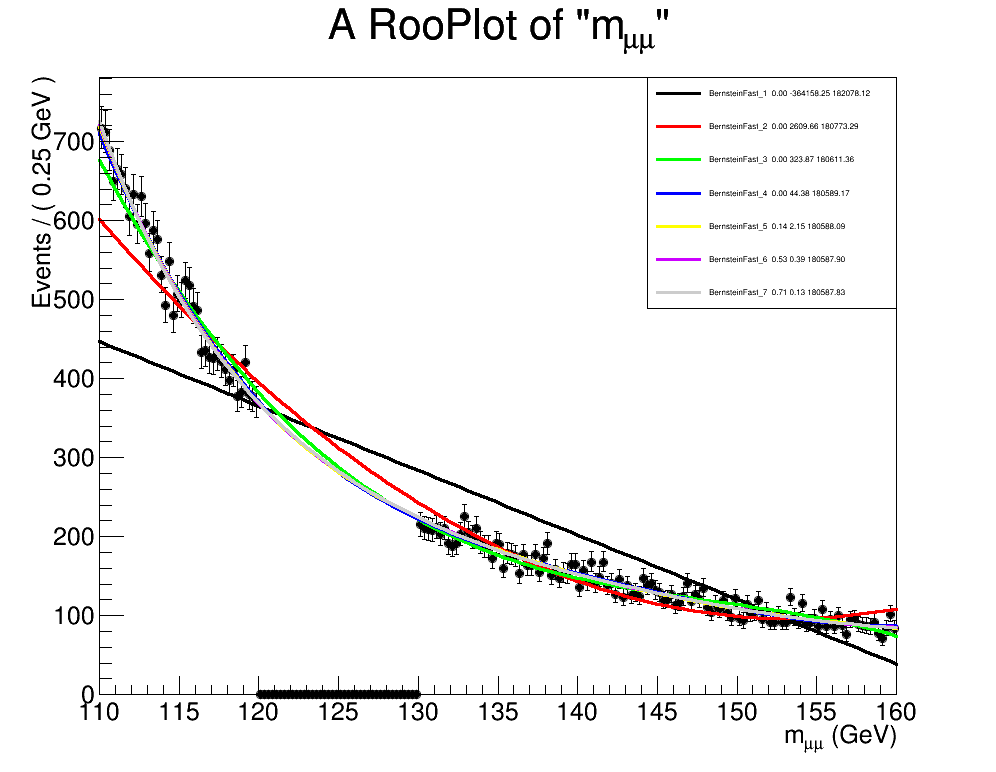
\includegraphics[width=0.45\textwidth]{figures/ch_higgs/ftest/baseline_110to160_p25GeV/ftest__01JetsTightBB__bernsteinFastModels.png}
     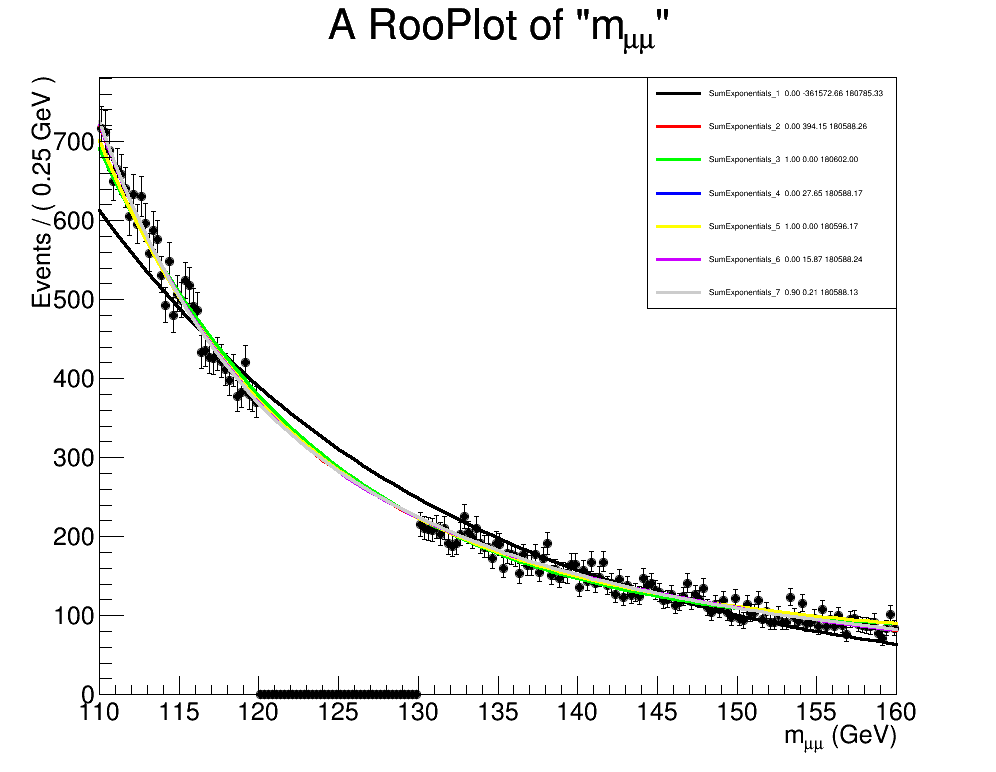
\includegraphics[width=0.45\textwidth]{figures/ch_higgs/ftest/baseline_110to160_p25GeV/ftest__01JetsTightBB__sumExpModels.png}
     \caption{}
     \label{fig:higgs_backgroundmodel_ftestexample}
 \end{figure}

 Figure~\ref{fig:higgs_backgroundmodel_ftestresults} provides examples of a summary of F-Test results upon which we can select a particular order for a given family.

 \begin{figure}[hbp]
     \centering
     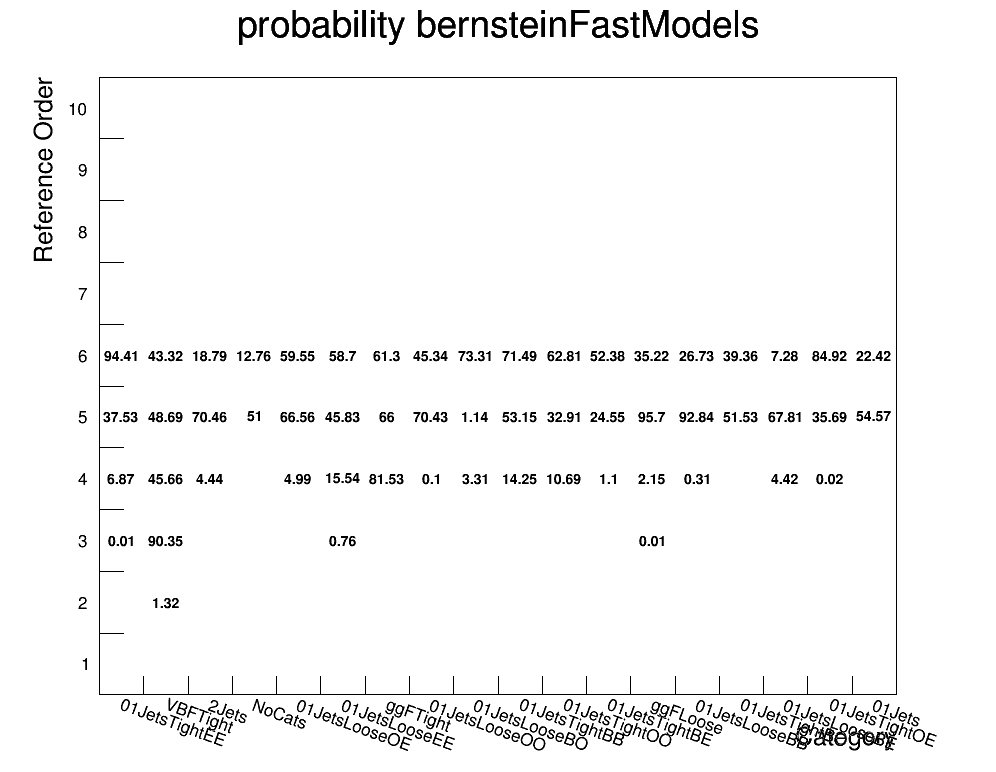
\includegraphics[width=0.45\textwidth]{figures/ch_higgs/ftest/baseline_110to160_p25GeV/ftestresults__probability__bernsteinFastModels.png}
     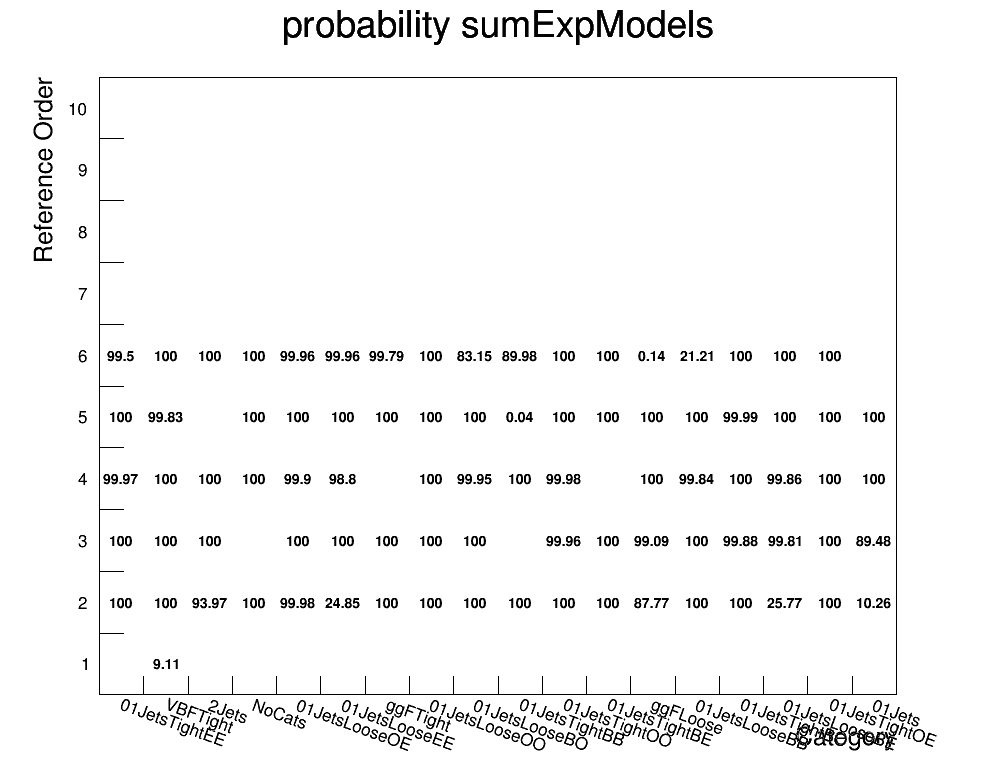
\includegraphics[width=0.45\textwidth]{figures/ch_higgs/ftest/baseline_110to160_p25GeV/ftestresults__probability__sumExpModels.png}
     \caption{}
     \label{fig:higgs_backgroundmodel_ftestresults}
 \end{figure}

\subsection{Higgs Combination} \label{subsection:higgs_analysis_signal}
%
% Ouline:
% - General Description of usage of Combine
% - InputFormat: Datacards and Workspaces
% - Playing with Asimov
% - Expected Limits
% - Maxlikelihood Fits
%
To perform statistical tests in order to extract physical quantities of interest, we employ Higgs Combination Package. It allows us to perform the tests for each category individually and combine all of the categories simultaneously as well. Given that we are performing a search of Standard Model Higgs Boson, the main objective is to improve (lower) the Exclusion Limits that we are to put on Standard Model Higgs Production Cross-Section with the data collected during Run II.

\subsubsection{Datacards and Workspaces}
The Combination Package expects several input items to perform the tests: datacards and workspaces with models. Datacard outlines our models, yields from data, signal and background processes. In the datacard, we also list all of the uncertainties or nuisances that will modify the yields of our models. Workspaces are the containers for the programmatically specified signal and background models. The detailed list of input items is the following:

\begin{itemize}
    \item Mass shapes for Data for each category.
    \item Background Models for each category. All of the Models come inside of an envelope (RooMultiPdf) as described in Section\textbf{FIXME}. The overall normalization for the background yield is floating and constrained by the Combination Package once the fit is performed.
    \item Signal Models for each category and for each production process. All of the model parameters come in as functions of the Higgs Mass. Given that we are performing a search, several mass hypotheses are tested. The overall normalization is frozen, however as a function of Higgs Mass.
    \item Nuisances. A number of systematic uncertainties influence our measurement (Integrated Luminosity, Pile-Up, etc...), therefore we provide multiplicative nuisance parameters that modify the signal yield.
\end{itemize}

\subsubsection{Validity Tests against Asimov}
The very first test of the validity of the model to be used is to perform the tests against the Asimov Dataset. The tests performed can summarized in the following procedure:

\begin{itemize}
    \item Given signal and background models we generate an Asimov dataset with some signal strength (typically it's 1).
    \item Perform the S+B fit to this Asimov should return back the expected signal strength with which this dataset has been generated.
    \item If a substantial bias has been observed, we can try profiling the likelihood (it's Negative Log-Likelihood to be exact) to see where the minimum of our test statistics is.
\end{itemize}

Figure~\ref{fig:higgs_analysis_asimovtests} provides examples of testing against Asimov Dataset. Mass spectrum on the left demonstrates the generated dataset overlaid with the fit. In the middle and on the right, examples of likelihood profiling vs the signal strength. important to point out that in the middle we have an example of a situation described previously - we observe a substantial amount of bias returned back from the fit of the Asimov generated with the injected signal strength of 1. The difference between middle and right is the granularity of the binning or number of points that are used to constrain the fit.

\begin{figure}[hbp]
     \centering
     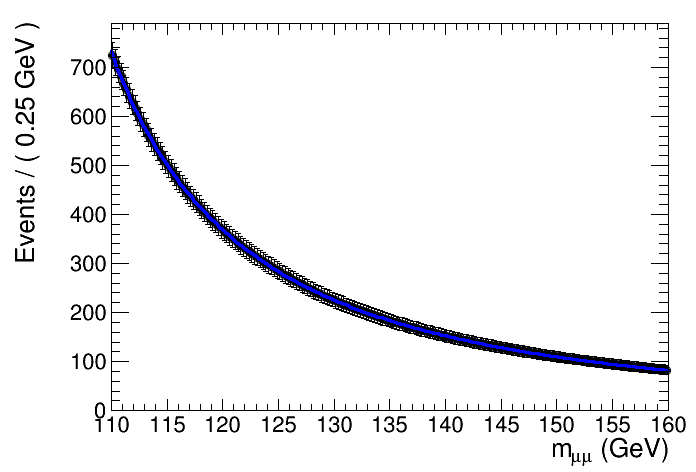
\includegraphics[width=0.3\textwidth]{figures/ch_higgs/asimovtests/cat6_x_fit_b.png}
     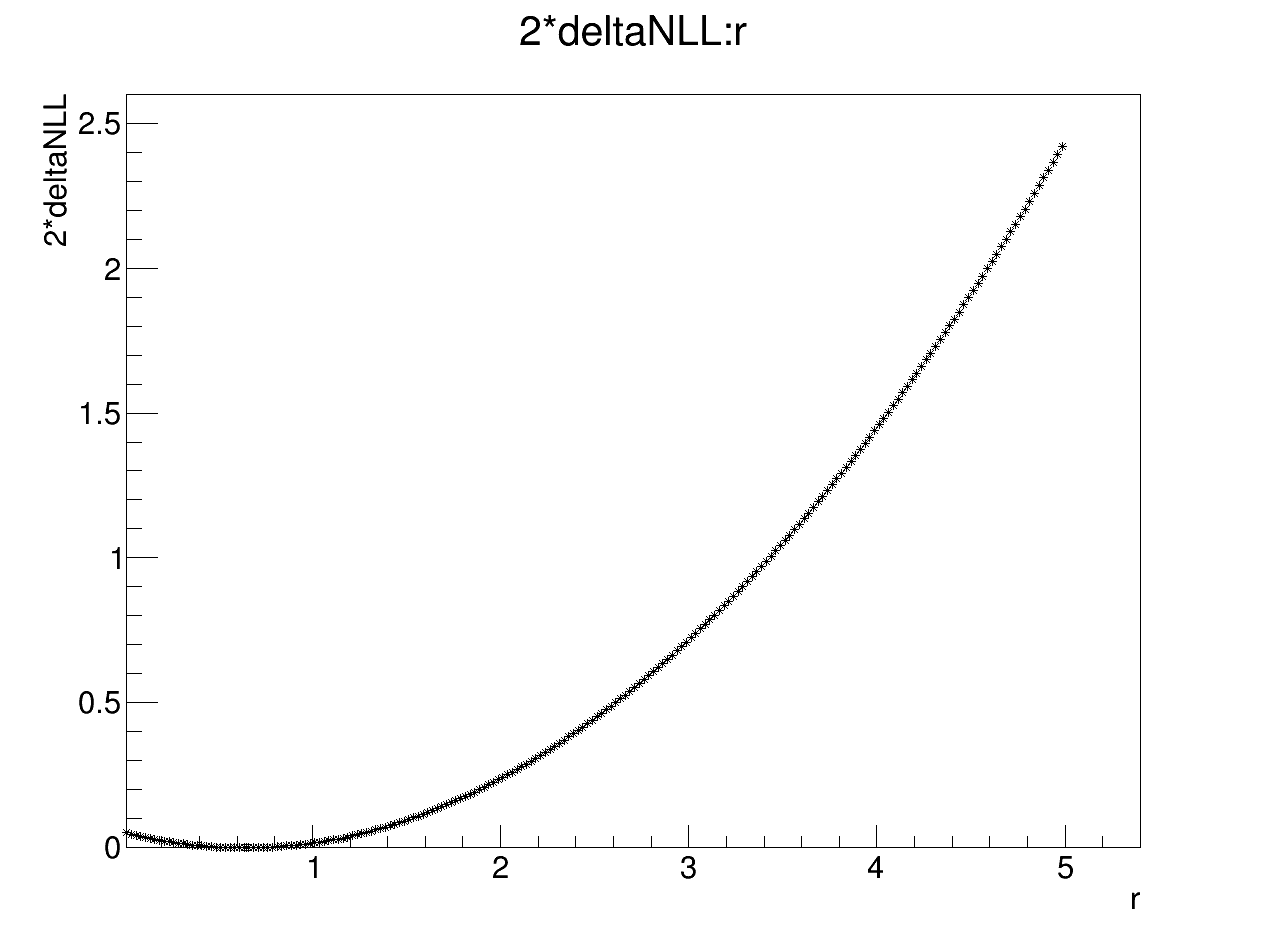
\includegraphics[width=0.3\textwidth]{figures/ch_higgs/asimovtests/NLL_asimovTest_1GeV.png}
     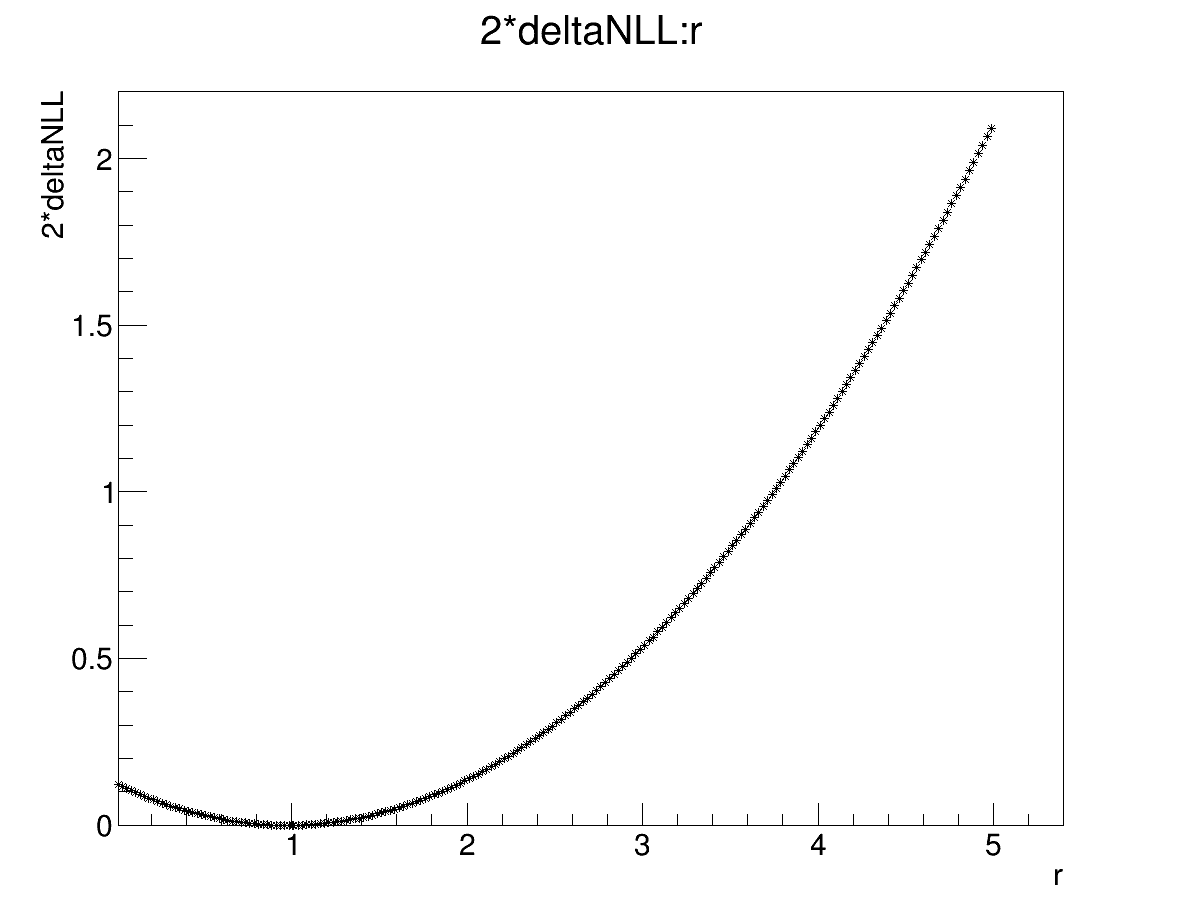
\includegraphics[width=0.3\textwidth]{figures/ch_higgs/asimovtests/NLL_asimovTest_p25GeV.png}
     \caption{}
     \label{fig:higgs_analysis_asimovtests}
 \end{figure}

\subsubsection{Exclusion Limits}
The most important physical quantity of interest that we are trying to compute and against which we optimize our analysis is the 95\% Confidence Level Exclusion Limits that we place on the production cross-section of the Standard Model Higgs Boson. Limits are computed using Asymptotic approximation.

Figures~\ref{fig:higgs_analysis_limitsexample} show examples of Exclusion Limits computed using Asymptotic Approximation. The left plot shows limits for Higgs Mass of 125 GeV only but across all of the categories and various combinations. The right one shows Exclusion Limits as a function of the probed Higgs Mass and for a combination of all of the categories.

\begin{figure}[hbp]
     \centering
     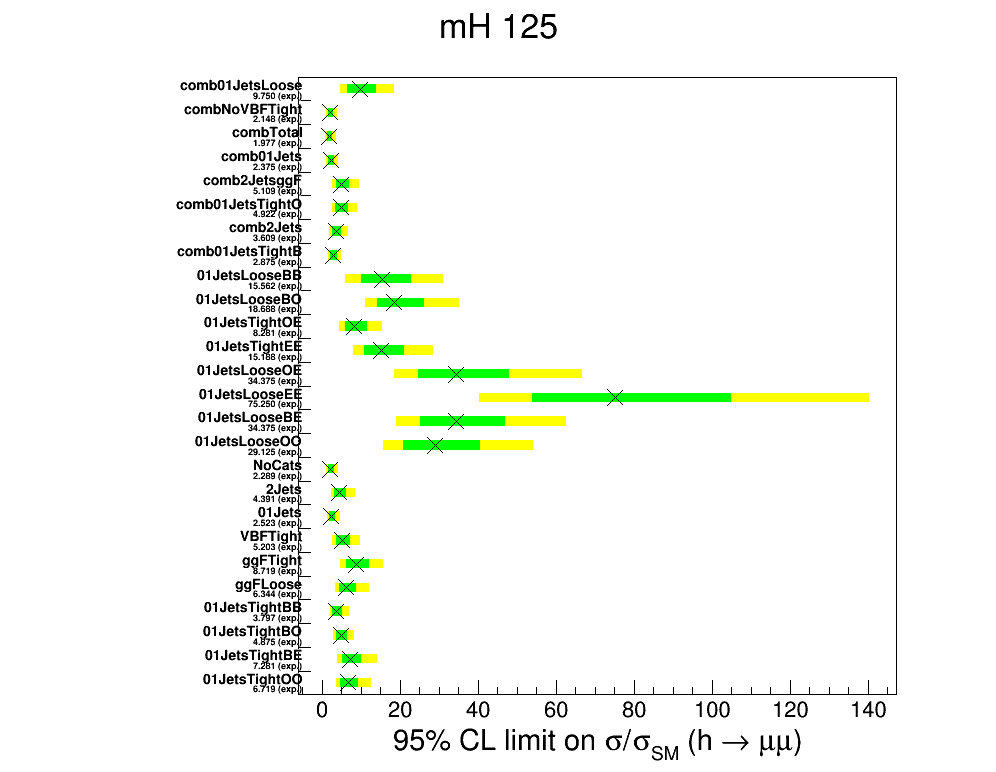
\includegraphics[width=0.45\textwidth]{figures/ch_higgs/limits/examples/limitsByMass__125__TripleGaus.png}
      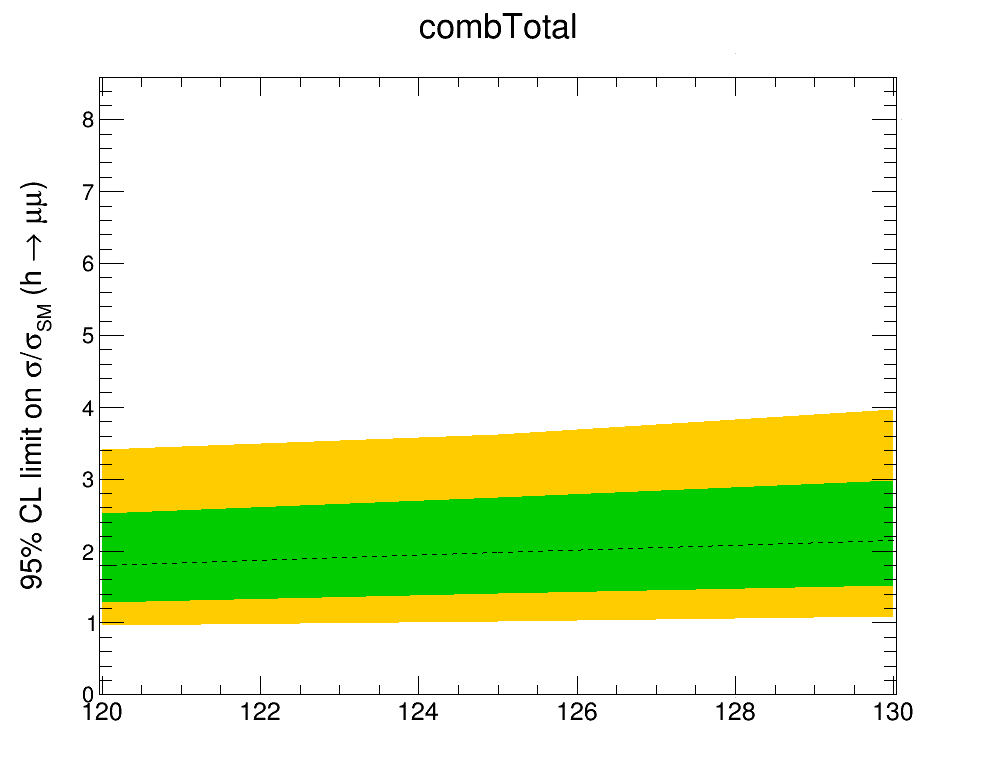
\includegraphics[width=0.45\textwidth]{figures/ch_higgs/limits/examples/limitsByCategory__combTotal__TripleGaus.png}
     \caption{}
     \label{fig:higgs_analysis_limitsexample}
 \end{figure}